% -*- mode: latex; ispell-local-dictionary: "en_GB" -*-

\documentclass[xcolor={usenames,dvipsnames}]{beamer}
\usepackage[utf8x]{inputenc}

\mode<presentation>
{
  \usetheme{Singapore}
  \usecolortheme{rose}
  %\setbeamercovered{transparent}
  \setbeamercovered{invisible}
  \setbeamercolor*{alerted text}{parent=titlelike}
}
\renewcommand{\emph}[1]{\alert{#1}}


%%% Packages %%%

% Use T1 and a modern font family for better support of accents, etc.
\usepackage[T1]{fontenc}
\usepackage{palatino}  % Palatino

% Language support
\usepackage[english]{babel}

% Support for easily changing the enumerator in
% enumerate-environments.
\usepackage{enumerate}

% Support for importing images
%\usepackage{graphicx}

% Use hyperlinks
\usepackage{hyperref}

% Don't load xcolors package in beamer: use document class option
% instead...
%\usepackage[usenames,dvipsnames]{xcolor}

% Use colors in tables
%\usepackage[pdftex]{colortbl}

% My personal list of commonly used math packages and macros
\usepackage{mathcommon}

% More math symbols (e.g. double-brackets: \llbracket, \rrbracket)
\usepackage{stmaryrd}

% A nice monospace font for listings, etc.
\usepackage[scaled]{beramono}
%\usepackage{inconsolata}

%\colorlet{Insertion}{NavyBlue}
\colorlet{Insertion}{blue}
\colorlet{Modification}{ForestGreen}
\colorlet{VariableEdge}{Cyan}
\colorlet{ImportantPath}{Cerulean}
\colorlet{SelectorEdge}{Plum}
\colorlet{LightGrey}{gray!40}
\colorlet{LightGreen}{green!20}


% Scala listings.  Use colored Scala style by default.
\usepackage{lstscala}
\lstset{
  style=scala-color,
  basicstyle=\footnotesize\tt,
  otherkeywords={do,od,nil},
  moredelim=**[is][\color{Insertion}]{@}{@},
  moredelim=**[is][\color{Modification}]{>}{<}}
\lstnewenvironment{lstscalasmall}{%
  \lstset{style=scala-color,basicstyle=\scriptsize\tt}}{}

% Algorithms/pseud-ocode typesetting
%\usepackage[ruled,vlined,linesnumbered]{algorithm2e}
%\usepackage[slide,vlined,linesnumbered]{algorithm2e}
%\usepackage{float}

% Using TikZ for diagrams
\usepackage{tikz}
\usetikzlibrary{arrows,fit,matrix,positioning,decorations.pathreplacing}
\usepackage{tikz-cd} % for CM-arrow tips.

% Don't use externalize with gradients!!!
%\usetikzlibrary{external,arrows,fit,matrix,positioning}
%\tikzexternalize % Activate externalizing TikZ graphics.

% Support per-slide PGF/TikZ keys (http://tex.stackexchange.com/a/6155)
\tikzset{onslide/.code args={<#1>#2}{%
  \only<#1>{\pgfkeysalso{#2}} % \pgfkeysalso doesn't change the path
}}

\newcommand{\TODO}[1]{\texttt{\textcolor{YellowOrange}{(#1)}}}

\newcommand\defeq{\stackrel{\mathclap{\tiny\mbox{def}}}{=}}

\newcommand{\transformer}[2]{$\llbracket$ \lstinline@#1@
  $\rrbracket_{\mathcal{#2}}$}
\newcommand{\transformerDSG}[1]{\transformer{#1}{DSG}}
\newcommand{\transformerSSG}[1]{\transformer{#1}{SSG}}
\newcommand{\mtransformer}[2]{\llbracket #1 \rrbracket_{\mathcal{#2}}}
\newcommand{\mtransformerDSG}[1]{\mtransformer{#1}{DSG}}
\newcommand{\mtransformerSSG}[1]{\mtransformer{#1}{SSG}}

%%%% Custom macros %%%%
\newif\ifcompileTreeSlides
%\compileTreeSlidesfalse
\compileTreeSlidestrue

%%% Document info %%%

\title{Solving Shape-Analysis Problems in Languages with Destructive Updating}

\subtitle{SAV Presentation}

\author[Sagiv~et~al.]{%
  {\small Authors}\\ \vspace{1ex}
  Molly Sagiv, Thomas W. Reps, Reinhard Wilhelm \\
  \vspace{1em}
  {\small Presenters}\\ \vspace{1ex}
  Marco Antognini, Sandro Stucki
}

% \institute[LAMP, Oracle]{%
%   \inst{1} LAMP, EPFL \and%
%   \inst{2} Oracle Labs}

% Logos
% \logo{
%   \includegraphics[height=7mm]{somelogo.png}\hspace{1mm}
%   \includegraphics[height=7mm]{someotherlogo}
% }

% To show the TOC at the beginning of each section, uncomment this:
% \AtBeginSection[]
% {
%   \begin{frame}<beamer>{Outline}
%     \tableofcontents[currentsection]
%   \end{frame}
% }

% To show the TOC at the beginning of each subsection, uncomment this:
% \AtBeginSubsection[]
% {
%   \begin{frame}<beamer>{Outline}
%     \tableofcontents[currentsection,currentsubsection]
%   \end{frame}
% }


% To uncover everything in a step-wise fashion, uncomment this:
% \beamerdefaultoverlayspecification{<+->}

\setbeamertemplate{footline}[frame number]

\date{%
  \vspace{-1em}
  \small May 2015\\[2em]
  
\includegraphics[height=7mm]{img/epfl-logo}}


%%% Start of the actual document %%%

\begin{document}

\begin{frame}
  \titlepage
\end{frame}

% Short-cut for inline listings using "@" (must come after "\titlepage")
\lstMakeShortInline[%
  style=scala-color,%
  flexiblecolumns=false,%
  mathescape=false,%
  basicstyle=\color{blue!30!darkgray}\tt]@


% No outline, too short a talk...
% \begin{frame}{Outline}
%   \tableofcontents
%   % You might wish to add the option [pausesections]
% \end{frame}

% No sections or subsections, too short a talk...
% \section{Motivation}
% \subsection*{}

\begin{frame}[fragile]{Motivation}
  Analyse the shape of heap allocated data structures.

  \vspace{1em}

  Verify that a program preserves shape properties such as:
  \begin{itemize}
  \item \textit{list-ness}
  \item \textit{circular list-ness}
  \item \textit{tree-ness}
  \end{itemize}

  \vspace{1em}

  This analysis algorithm can be used to find \emph{aliases}, and therefore to optimise code (no alias means it can be more easily parallelised).
\end{frame}

% CFG nodes. #1: node number, #2: statement.
\newcommand{\stmtmini}[1]{%
  \node[draw, minimum width=5em, minimum height=1.25em, inner sep=1.5pt] (#1)
  {\lstinline[basicstyle=\tiny\ttfamily]@#1@};}

\newcommand{\stmt}[2]{%
  \node{$v_{#1}$}; \&
  \node[draw, minimum width=14em, minimum height=1.25em, inner sep=1.5pt] (v#1)
  {\lstinline[basicstyle=\tiny\ttfamily]@#2@};}
  
\newcommand{\stmtgroup}[3]{%
  \draw [thick, ImportantPath, decorate, decoration={brace}]([xshift=3em]#1.north east) -- ([xshift=3em]#2.south east) node[black, midway, xshift=0.5em, anchor=west] {#3};}

\begin{frame}[fragile]{List Reversal -- Normalisation}
  \begin{columns}[T]
	  \column{.5\textwidth}
	  \begin{onlyenv}<1>
	  \begin{lstlisting}[mathescape=true]
	  // x points to an unshared list
	  y := nil
	  while x $ \neq $ nil do

	    t := y

	    y := x



	    x := x.cdr

	    y.cdr := t
	  od

	  t := nil
	  \end{lstlisting}
	  \end{onlyenv}
	  \begin{onlyenv}<2->
	  \begin{lstlisting}[mathescape=true]
	  // x points to an unshared list
	  y := nil
	  while x $ \neq $ nil do
	    @t := nil@
	    t := y
	    @y := nil@
	    y := x
	    @t$\color{Insertion}_1$ := nil@
	    @t$\color{Insertion}_1$ := x.cdr@
	    @x := nil@
	    >x := t$\color{Modification}_1$<
	    @y.cdr := nil@
	    y.cdr := t
	  od
	  @t$\color{Insertion}_1$ := nil@
	  t := nil
	  \end{lstlisting}
        \end{onlyenv}
        \column{.5\textwidth}
        \pause\pause
        \begin{tikzpicture}[ampersand replacement=\&, >=latex]
          \tiny
          \matrix[row sep=.75em] {
            \stmt{1}{y := nil} \\
            \stmt{2}{} \\
            \stmt{3}{t := nil} \\
            \stmt{4}{t := y} \\
            \stmt{5}{y := nil} \\
            \stmt{6}{y := x} \\
            \stmt{7}{t$_1$ := nil} \\
            \stmt{8}{t$_1$ := x.cdr} \\
            \stmt{9}{x := nil} \\
            \stmt{10}{x := t$_1$} \\
            \stmt{11}{y.cdr := nil} \\
            \stmt{12}{y.cdr := t} \\
            \stmt{13}{t$_1$ := nil} \\
            \stmt{14}{t := nil} \\
            \stmt{15}{} \\
          };
          \path[->]
          (v1.north) +(0,+1em) edge (v1)
          (v1) edge (v2)
          (v2) edge (v3)
          (v3) edge (v4)
          (v4) edge (v5)
          (v5) edge (v6)
          (v6) edge (v7)
          (v7) edge (v8)
          (v8) edge (v9)
          (v9) edge (v10)
          (v10) edge (v11)
          (v11) edge (v12)
          (v13) edge (v14)
          (v14) edge (v15);
          \draw[->] ([yshift=.5ex]v2.east) -- +(2em, 0) |- (v13);
          \draw[->] (v12.east) -- +(1em, 0) |- ([yshift=-.5ex]v2);
        \end{tikzpicture}
  \end{columns}
\end{frame}


%%%% The following is a crazy TikZ slide combining tree/graph drawing
%%%% code, etc.

\newcommand{\celldraw}[1]{#1!80!black!80!white}%
\newcommand{\cellfill}[1]{#1!80!black!30!white}%

% Basic style of a cell box.
\tikzstyle{cellbox}=[rectangle, thick, draw=\celldraw{#1}, top color=white,%
  bottom color=\cellfill{#1}, minimum width=2em, minimum height=1em,
  inner sep=0]

% The matrix style underlying graphs.
\tikzstyle{graph}=[matrix, row sep=1pt, column sep=.5em, node distance=0pt,%
  nodes={anchor=center}]

% Basic style for variable labels.
\tikzstyle{labelnode}=[font=\tiny, node distance=.6em, inner sep=1pt]

% Style for transformer arrow tips.
\tikzstyle{trans}=[-cm to]

% Basic cell.  The first argument is the name of the node (in TeX,
% e.g. "xy"), the second one is its printed name (e.g. "n_{x, y}").
% The third argument determines the color.  The optional argument
% contains extra node parameters (e.g. minimum width=1em creates cell
% that is less wide).
\newcommand{\cell}[4][]{%
  \node[cellbox=#4, #1] (#2) {};
  \draw[draw=\celldraw{#4}, semithick] (#2.north) -- (#2.south);
  \path (#2.west) -- coordinate[midway] (#2-car) (#2.center);
  \path (#2.east) -- coordinate[midway] (#2-cdr) (#2.center);
  \node[font=\tiny, below=of #2.south west, anchor=north west, inner sep=1pt]
  {$#3$};}%

% A basic cons cell with a circle in the "cdr" box.  Arguments are the
% same as for \cell.
\newcommand{\cons}[4][]{%
  \cell[#1]{#2}{#3}{#4}%
  \node[circle, fill=black, inner sep=.75pt] at (#2-cdr) {};}%

% A concrete (green) cons cell.
\newcommand{\ccons}[3][]{\cons[#1]{#2}{#3}{green}}

% A concrete unreachable cons cell - ready to be garbage collected
\newcommand{\cucons}[3][]{\cons[#1]{#2}{#3}{LightGreen}}
% pattern=soft crosshatch ?

% An abstract (blue) cons cell.
\newcommand{\acons}[3][]{\cons[#1]{#2}{n_{#3}}{blue}}

% A shared (red) cons cell.
\newcommand{\scons}[3][]{\cons[#1]{#2}{n_{#3}}{red}}

% A "transparent" cons cell (can be used as a placeholder).
\newcommand{\tcell}[1][]{
  \node[rectangle, minimum width=2em, minimum height=1em, inner sep=0,
  #1] {};}

% A named "transparent" cons cell (can be used as a placeholder).
\newcommand{\ntcell}[2][]{
  \node[rectangle, minimum width=2em, minimum height=1em, inner sep=0,
  #1] (#2) {};
  \path (#2.west) -- coordinate[midway] (#2-car) (#2.center);
  \path (#2.east) -- coordinate[midway] (#2-cdr) (#2.center);}


% Variable label and edge. Arguments are position, node and label text.
\newcommand{\vlabel}[3]{%
  \node[labelnode, #1=of #2] {$#3$} edge (#2);}%

% example: \vlabelwy{xy}{x}{1mm}
\newcommand{\vlabelwy}[3]{%
  \node[labelnode, yshift=#3, left=of #1] {$#2$} edge ([yshift=#3]#1.west);}%

% example: \vlabelnx{xy}{x}{1mm}
\newcommand{\vlabelnx}[3]{%
  \node[labelnode, xshift=#3, above=of #1] {$#2$} edge ([xshift=#3]#1.north);}%

% Draws a "transformer" arrow.
\newcommand{\transarrow}[3]{%
  \draw[trans] ($(#1.east)+(1em,0)$) -- node[above]{\normalsize #2}
  ($(#3.west)+(-1.5em,0)$);}

% Draws a vertical "transformer" arrow.
\newcommand{\vtransarrow}[4][left]{%
  \draw[trans] ($(#2.south)+(0,-.5em)$) -- node[#1]{\normalsize #3}
  ($(#4.north)+(0,.5em)$);}


\ifcompileTreeSlides



\begin{frame}[fragile]{Shape-Graph $SG = \tpl{E_v, E_s}$}

	%\emph{Not} to be confused by a program control flow graph $G = \tpl{V, A}$
	%\vspace{1em}
	
	What is a \textbf{shape-graph}?

	\begin{itemize}
	\item directed graph with nodes and edges
	\item nodes are called \textcolor{Green}{\textbf{shape-nodes}}
		\begin{itemize}
		\item[$\circ$] runtime locations, i.e. heap memory, or \textit{cons-cells}
		\item[$\circ$] implicitly defined by edges and $shape\_nodes(SG)$
		\end{itemize}
	\item edges are divided into 2 categories:
		\begin{itemize}
    	\item[$\circ$] \textcolor{VariableEdge}{$E_v$: \textbf{variable-edges}} of the form $ \left[x, n\right] $
    	\item[$\circ$] \textcolor{SelectorEdge}{$E_s$: \textbf{selector-edges}} of the form $ \tpl{s, sel, t} $
		\end{itemize}
	\end{itemize}

	\begin{center}
    \begin{tikzpicture}[semithick,
      ampersand replacement=\&, every edge/.append style={->}, >=latex]
      \Large % <-- determines scale of diagram. try \LARGE, \Huge, \small...

      % Matrix for arranging graph nodes.  You can set the overall
      % spacing through "row sep" and "column sep" or add and remove
      % horizontal or vertical space in brackets after \& and \\.
      \matrix[graph, column sep=1em] (g1) %<-- general column spacing
      {
        \ccons[minimum width=1em]{l1}{l_1} \&
        \ccons[minimum width=1em]{l2}{l_2} \&
        \ccons[minimum width=1em]{l3}{l_3} \\
      };

      % Selector edges.
      \path[->]
      (l1-cdr) edge[SelectorEdge] (l2)
      (l2-cdr) edge[SelectorEdge] (l3);

      % Variable egdes.
      %\vlabel{left}{l1}{x} % need color on edge:
      \node[labelnode, left=of l1] {$x$} edge[VariableEdge] (l1);
    \end{tikzpicture}
  \end{center}

	%$n, s, t, l_1, l_2$ and $l_3$ are shape-nodes, $x$ a program variable and $sel \in \left\{ car, cdr \right\}$

\end{frame}

\begin{frame}[fragile]{$DSG$: Deterministic Shape-Graph}
%  $E_v$ and $E_s$ are also used as functions:
%  \begin{itemize}
%  \item $E_v(x) \defeq \left\{ n \mid \left[x, n\right] \in E_v \right\}$
%  \item $E_s(s, sel) \defeq \left\{ t \mid \tpl{s, sel, t} \in E_s \right\}$
%  \end{itemize}
%
%  \vspace{1em}

  A shape-graph is \emph{deterministic} if
  \begin{enumerate}
  \item no variable points to more than one node%: $ |E_v(*)| \leq 1$
  \item no node has a selector pointing to more than one node%: $ |E_s(*, *)| \leq 1$
  \end{enumerate}

  \vspace{1em}  
  In other words:\\
  \hspace{1.5em} It is deterministic when edges are behaving like \emph{pointers}.
\end{frame}


\begin{frame}[fragile]{$gc$: Garbage Collection}
  The $gc$ function removes runtime location that are not reachable from any program variable:

  \vspace{1em}

  $ gc: SG \to SG $\\
  $ gc\left(\tpl{E_v, E_s} \right) \defeq \tpl{E_v, E'_s} $ where $ E'_s \subseteq E_s $ and $ \tpl{s, sel, t} \in E'_s $ if and only if there exists $ \left[ x, r \right] \in E_v $ such that there is a path of selector-edges in $ E_s $ from $r$ to $s$.

	\begin{center}
    \begin{tikzpicture}[semithick,
      ampersand replacement=\&, every edge/.append style={->}, >=latex]
      \Large % <-- determines scale of diagram. try \LARGE, \Huge, \small...

      // Initial graph
      \matrix[graph, column sep=1em] (lhs) at (-8em, 0)
      {
        \ccons[minimum width=1em]{l1}{l_1} \&
        \ccons[minimum width=1em]{l2}{l_2} \\
        \ccons[minimum width=1em]{l3}{l_3} \&
        \ccons[minimum width=1em]{l4}{l_4} \&
        \ccons[minimum width=1em]{l5}{l_5} \\
      };

      % Selector edges.
      \path[->]
      (l1-cdr) edge (l2)
      (l2-cdr) edge (l5)
      (l3-cdr) edge (l4)
      (l4-cdr) edge (l5);

      % Variable egdes.
      \vlabel{left}{l1}{x}
      
      % After applying gc
      \matrix[graph, column sep=1em] (rhs) at (7em, 0)
      {
        \ccons[minimum width=1em]{l1}{l_1} \&
        \ccons[minimum width=1em]{l2}{l_2} \\
        \& \&
        \ccons[minimum width=1em]{l5}{l_5} \\
      };

      % Selector edges.
      \path[->]
      (l1-cdr) edge (l2)
      (l2-cdr) edge (l5);

      % Variable egdes.
      \vlabel{left}{l1}{x}
      
      % Transformer arrow
      \transarrow{lhs}{$gc$}{rhs}
    \end{tikzpicture}
  \end{center}
\end{frame}


\begin{frame}[fragile]{$DSG$ Transformers}
  A program statement is represented as a transform function on $DSG$, denoted \transformerDSG{st}.

  \vspace{1em}

  Thanks to program normalisation, there are only 6 statements and they are simple:

  \begin{enumerate}
  \item \transformerDSG{x := nil}
  \item \transformerDSG{x.sel := nil}
  \item \transformerDSG{x := new}
  \item \transformerDSG{x := y}
  \item \transformerDSG{x := y.sel}
  \item \transformerDSG{x.sel := y}
  \end{enumerate}
\end{frame}

\begin{frame}[fragile]{$DSG$ Transformers: 1}
  \begin{flalign*}
    & \text{\transformerDSG{x := nil}} \left( \tpl{E_v, E_s} \right) & \\
    & \quad \quad \quad \quad \quad \quad \defeq \tpl{E_v - \left\{\left[ \texttt{x}, * \right]\right\}, E_s}
  \end{flalign*}

  \vspace{1em}

  \begin{center}
    \begin{tikzpicture}[semithick, ampersand replacement=\&,%
      every edge/.append style={->}, >=latex]
      \Large

      \matrix[graph, column sep=1em] (lhs) at (-8em, 0)
      {
        \ccons[minimum width=1em]{l1}{l_1} \&
        \ccons[minimum width=1em]{l2}{l_2} \&
        \ccons[minimum width=1em]{l3}{l_3} \\
      };

      % Selector edges.
      \path[->]
      (l1-cdr) edge (l2)
      (l2-cdr) edge (l3);

      % Variable egdes.
      \vlabel{left}{l1}{x}
      \vlabel{above}{l2}{y}

      \matrix[graph, column sep=1em] (rhs) at (7em, 0)
      {
        \cucons[minimum width=1em]{l1}{l_1} \&
        \ccons[minimum width=1em]{l2}{l_2} \&
        \ccons[minimum width=1em]{l3}{l_3} \\
      };

      % Selector edges.
      \path[->]
      (l2-cdr) edge (l3);

      % Variable egdes.
      \vlabel{above}{l2}{y}

      % Transformer arrow
      \transarrow{lhs}{\transformerDSG{x := nil}}{rhs}
    \end{tikzpicture}
  \end{center}

  NB: $gc$ can do some cleaning.
\end{frame}


\begin{frame}[fragile]{$DSG$ Transformers: 2}
  \begin{flalign*}
    & \text{\transformerDSG{x.sel := nil}} \left( \tpl{E_v, E_s} \right) & \\
    & \quad \quad \quad \quad \quad \quad \defeq \tpl{E_v, E_s - \left\{ \tpl{s, \texttt{sel}, *} \mid \left[\texttt{x},s\right] \in E_v \right\}}
  \end{flalign*}

  \vspace{1em}

  \begin{center}
    \begin{tikzpicture}[semithick,
      ampersand replacement=\&, every edge/.append style={->}, >=latex]
      \Large % <-- determines scale of diagram. try \LARGE, \Huge, \small...

      % BEFORE
      \matrix[graph, column sep=1em] (lhs) at (-8em, 0)
      {
        \ccons[minimum width=1em]{l1}{l_1} \&
        \ccons[minimum width=1em]{l2}{l_2} \&
        \ccons[minimum width=1em]{l3}{l_3} \\
      };

      % Selector edges.
      \path[->]
      (l1-cdr) edge (l2)
      (l2-cdr) edge (l3);

      % Variable egdes.
      \vlabel{left}{l1}{x}
      \vlabel{above}{l2}{y}
      
      % AFTER
      \matrix[graph, column sep=1em] (rhs) at (7em, 0)
      {
        \ccons[minimum width=1em]{l1}{l_1} \&
        \ccons[minimum width=1em]{l2}{l_2} \&
        \cucons[minimum width=1em]{l3}{l_3} \\
      };

      % Selector edges.
      \path[->]
      (l1-cdr) edge (l2);

      % Variable egdes.
      \vlabel{left}{l1}{x}
      \vlabel{above}{l2}{y}
      
      % Transformer arrow
      \transarrow{lhs}{\transformerDSG{y.cdr := nil}}{rhs}
    \end{tikzpicture}
  \end{center}
  
  NB: $gc$ can do some cleaning.
\end{frame}



\begin{frame}[fragile]{$DSG$ Transformers: 3}
  \begin{flalign*}
    & \text{\transformerDSG{x := new}} \left( \tpl{E_v, E_s} \right) & \\
    & \quad \quad \quad \quad \quad \quad \defeq \tpl{E_v \cup \left\{ \left[ \mbox{x}, \mbox{n}_{new} \right] \right\}, E_s}
  \end{flalign*}

  \vspace{1em}

  \begin{center}
    \begin{tikzpicture}[semithick,
      ampersand replacement=\&, every edge/.append style={->}, >=latex]
      \Large % <-- determines scale of diagram. try \LARGE, \Huge, \small...

      \matrix[graph, column sep=1em] (lhs) at (-8em, 0)
      {
        \ccons[minimum width=1em]{l1}{l_1} \&
        \ccons[minimum width=1em]{l2}{l_2} \&
        \ccons[minimum width=1em]{l3}{l_3} \\
      };

      % Selector edges.
      \path[->]
      (l1-cdr) edge (l2)
      (l2-cdr) edge (l3);

      % Variable egdes.
      \vlabel{left}{l1}{x}
      \vlabel{above}{l2}{y}
      
      \matrix[graph, column sep=1em] (rhs) at (7em, 0)
      {
        \ccons[minimum width=1em]{l1}{l_1} \&
        \ccons[minimum width=1em]{l2}{l_2} \&
        \ccons[minimum width=1em]{l3}{l_3} \&
        \ccons[minimum width=1em]{l4}{l_4} \\
      };

      % Selector edges.
      \path[->]
      (l1-cdr) edge (l2)
      (l2-cdr) edge (l3);

      % Variable egdes.
      \vlabel{left}{l1}{x}
      \vlabel{above}{l2}{y}
      \vlabel{above}{l4}{z}
      
      % Transformer arrow
      \transarrow{lhs}{\transformerDSG{z := new}}{rhs}
    \end{tikzpicture}
  \end{center}
  
  \vphantom{NB: $gc$ can do some cleaning.}
\end{frame}



\begin{frame}[fragile]{$DSG$ Transformers: 4}
  \begin{flalign*}
    & \text{\transformerDSG{x := y}} \left( \tpl{E_v, E_s} \right) & \\
    & \quad \quad \quad \quad \quad \quad \defeq \tpl{E_v \cup \left\{ \left[ \mbox{x}, \mbox{n} \right] \mid \left[ \mbox{y}, \mbox{n} \right] \in E_v \right\}, E_s}
  \end{flalign*}

  \vspace{1em}

  \begin{center}
    \begin{tikzpicture}[semithick,
      ampersand replacement=\&, every edge/.append style={->}, >=latex]
      \Large % <-- determines scale of diagram. try \LARGE, \Huge, \small...

      \matrix[graph, column sep=1em] (lhs) at (-8em, 0)
      {
        \ccons[minimum width=1em]{l1}{l_1} \&
        \ccons[minimum width=1em]{l2}{l_2} \&
        \ccons[minimum width=1em]{l3}{l_3} \\
      };

      % Selector edges.
      \path[->]
      (l1-cdr) edge (l2)
      (l2-cdr) edge (l3);

      % Variable egdes.
      \vlabel{left}{l1}{x}
      \vlabel{above}{l2}{y}
      
      \matrix[graph, column sep=1em] (rhs) at (7em, 0)
      {
        \ccons[minimum width=1em]{l1}{l_1} \&
        \ccons[minimum width=1em]{l2}{l_2} \&
        \ccons[minimum width=1em]{l3}{l_3} \\
      };

      % Selector edges.
      \path[->]
      (l1-cdr) edge (l2)
      (l2-cdr) edge (l3);

      % Variable egdes.
      \vlabel{left}{l1}{x}
      \vlabel{above}{l1}{z}
      \vlabel{above}{l2}{y}
      
      % Transformer arrow
      \transarrow{lhs}{\transformerDSG{z := x}}{rhs}
    \end{tikzpicture}
  \end{center}
  
  \vphantom{NB: $gc$ can do some cleaning.}
\end{frame}



\begin{frame}[fragile]{$DSG$ Transformers: 5}
  \begin{flalign*}
	  & \text{\transformerDSG{x := y.sel}} \left( \tpl{E_v, E_s} \right) & \\
	  & \quad \quad \quad \quad \quad \quad \defeq \tpl{E_v \cup \left\{ \left[ \mbox{x}, \mbox{t} \right] \mid \left[ \mbox{y}, \mbox{s} \right] \in E_v \wedge \tpl{\mbox{s}, \mbox{sel}, \mbox{t}} \in E_s \right\}, E_s}
  \end{flalign*}

  \vspace{1em}

  \begin{center}
    \begin{tikzpicture}[semithick,
      ampersand replacement=\&, every edge/.append style={->}, >=latex]
      \Large % <-- determines scale of diagram. try \LARGE, \Huge, \small...

      \matrix[graph, column sep=1em] (lhs) at (-8em, 0)
      {
        \ccons[minimum width=1em]{l1}{l_1} \&
        \ccons[minimum width=1em]{l2}{l_2} \&
        \ccons[minimum width=1em]{l3}{l_3} \\
      };

      % Selector edges.
      \path[->]
      (l1-cdr) edge (l2)
      (l2-cdr) edge (l3);

      % Variable egdes.
      \vlabel{left}{l1}{x}
      \vlabel{above}{l2}{y}
      
      \matrix[graph, column sep=1em] (rhs) at (7em, 0)
      {
        \ccons[minimum width=1em]{l1}{l_1} \&
        \ccons[minimum width=1em]{l2}{l_2} \&
        \ccons[minimum width=1em]{l3}{l_3} \\
      };

      % Selector edges.
      \path[->]
      (l1-cdr) edge (l2)
      (l2-cdr) edge (l3);

      % Variable egdes.
      \vlabel{left}{l1}{x}
      \vlabel{above}{l2}{y}
      \vlabel{above}{l3}{z}
      
      % Transformer arrow
      \transarrow{lhs}{\transformerDSG{z := y.cdr}}{rhs}
    \end{tikzpicture}
  \end{center}
  
  \vphantom{NB: $gc$ can do some cleaning.}
\end{frame}



\begin{frame}[fragile]{$DSG$ Transformers: 6}
  \begin{flalign*}
    & \text{\transformerDSG{x.sel := y}} \left( \tpl{E_v, E_s} \right) & \\
    & \quad \quad \quad \quad \quad \quad \defeq \tpl{E_v, E_s \cup \left\{ \tpl{\mbox{s}, \mbox{sel}, \mbox{t}} \mid \left[ \mbox{x}, \mbox{s} \right] \in E_v \wedge \left[ \mbox{y}, \mbox{t} \right] \in E_v \right\}}
  \end{flalign*}

  \vspace{1em}
  
  \begin{center}
    \begin{tikzpicture}[semithick,
      ampersand replacement=\&, every edge/.append style={->}, >=latex]
      \Large % <-- determines scale of diagram. try \LARGE, \Huge, \small...

      \matrix[graph, column sep=1em] (lhs) at (-8em, 0)
      {
        \ccons[minimum width=1em]{l1}{l_1} \&
        \ccons[minimum width=1em]{l2}{l_2} \&
        \ccons[minimum width=1em]{l3}{l_3} \\
      };

      % Selector edges.
      \path[->]
      (l1-cdr) edge (l2);

      % Variable egdes.
      \vlabel{left}{l1}{x}
      \vlabel{above}{l2}{y}
      \vlabel{above}{l3}{z}
      
      \matrix[graph, column sep=1em] (rhs) at (7em, 0)
      {
        \ccons[minimum width=1em]{l1}{l_1} \&
        \ccons[minimum width=1em]{l2}{l_2} \&
        \ccons[minimum width=1em]{l3}{l_3} \\
      };

      % Selector edges.
      \path[->]
      (l1-cdr) edge (l2)
      (l2-cdr) edge (l3);

      % Variable egdes.
      \vlabel{left}{l1}{x}
      \vlabel{above}{l2}{y}
      \vlabel{above}{l3}{z}
      
      % Transformer arrow
      \transarrow{lhs}{\transformerDSG{y.cdr := z}}{rhs}
    \end{tikzpicture}
  \end{center}
  
  \vphantom{NB: $gc$ can do some cleaning.}
\end{frame}

\begin{frame}[fragile]{Collecting Semantics}
  Each DSG models one runtime behaviour (of many).

  \vspace{1em}

  We need a tool to perform analysis on \textbf{all} possible execution paths, not just one.

  \vspace{2em}

  Hence the collecting function $cv: V \to 2^{DSG}$ \\
  $cv(v) \defeq \{ $ \transformerDSG{st($v_k$)} $ ( \cdots ( $ \transformerDSG{st($v_1$)} $ ( \tpl{\emptyset, \emptyset} ))) \mid $ \\
  \hspace{16em} $ \left[ v_1, \ldots, v_k \right] \in pathsTo(v) \} $

  \vspace{2em}

  $V$ is the vertex set of the \textit{regular} control flow graph $G = \tpl{V, A}$.
\end{frame}


\begin{frame}{Abstraction, Abstractly}
  \vspace{-0.5em}
  \begin{center}
    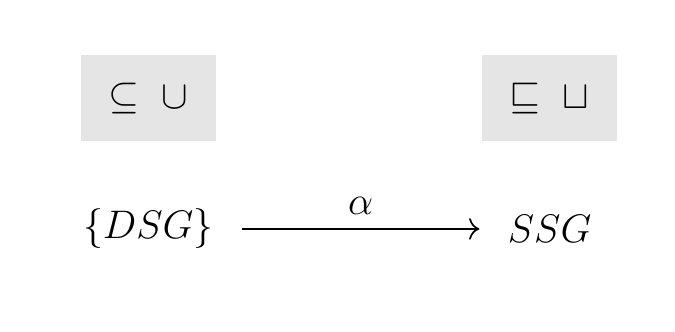
\begin{tikzpicture}[semithick,ampersand replacement=\&, >=cm to]
      \Large

      % Shape graphs
      \matrix[matrix, column sep=6em, row sep=3em, inner sep=10pt] {
        \uncover<2->{\node[fill=gray!20!white] {$\subseteq \; \cup$};} \&
        \uncover<3->{\node[fill=gray!20!white]
          {$\sqsubseteq \; \sqcup$};} \\[-2em]
        \node (D) {$\phantom{\{} DSG \phantom{\}}$}; \&
        \uncover<3->{\node (S) {$SSG$};} \\
      };

      % Extra "set braces"
      \uncover<2->{\node at (D) {$\{ \phantom{DSG} \}$};}

      % Arrows.
      \uncover<3->{\draw[->] (D) -- node[above]{$\alpha$} (S);}
    \end{tikzpicture}
  \end{center}
  \pause\pause\pause

  \emph{Static shape graphs:} $SSG = \tpl{SG, is\_shared} $
  \begin{itemize}
  \item $SG$ is a shape graph
  \item $is\_shared\colon shape\_nodes(SG) \to \set{T, F}$

    is a predicate identifying nodes that were shared in the DSG
  \end{itemize}
\end{frame}

% 6. abstraction function with SSG
%    - relation between quotient and alpha function(s)
\begin{frame}{Abstraction -- Helpers}
  \begin{itemize}
  \item Grouping nodes by variable labels
    \begin{align*}
      \alpha_s[DSG] &\colon shape\_nodes(DSG) \to \setof{n_X}{X
        \subseteq PVar}\\
      \alpha_s[DSG] &(r) \defeq n_{\setof{ x \in PVar }{[x, r] \in
          E_v}}
    \end{align*}
  \item Initialisation of the sharing predicate
    \begin{align*}
      induced\_is\_shared[DSG] &\colon shape\_nodes(DSG) \to \set{T, F}\\
      induced\_is\_shared[DSG] &(t) \defeq \abs{\set{\tpl{*, *, t} \in
          E_s}} \leq 2
    \end{align*}
  \item Projection (a.k.a.\ quotienting) of SGs with respect to $f$
    \begin{align*}
      \tpl{SG, p} \downarrow f
    \end{align*}
  \end{itemize}
\end{frame}

% 6. abstraction function with SSG
%    - relation between quotient and alpha function(s)
\begin{frame}{Abstraction}
  \begin{itemize}
  \item Projection/quotient of a single DSG
    \begin{align*}
      \hat{\alpha} &\colon \mathcal{DSG} \to \mathcal{SSG}\\
      \hat{\alpha} &(DSG) \defeq \tpl{DSG', induced\_is\_shared[DSG']}
      \downarrow \alpha_s[DSG']\\
      &\quad \text{where } DSG' = gc(DSG)
    \end{align*}
  \item Abstraction function
    \begin{align*}
      \alpha &\colon 2^{\mathcal{DSG}} \to \mathcal{SSG}\\
      \alpha &(S) \defeq \bigsqcup_{DSG \in S} \hat{\alpha}(DSG)
    \end{align*}
  \end{itemize}
\end{frame}

% 7. commutative diagram for [st]DSG / alpha / [st]SSG
\begin{frame}{Abstract Interpretation, Abstractly}
  \vspace{-0.5em}
  \begin{center}
    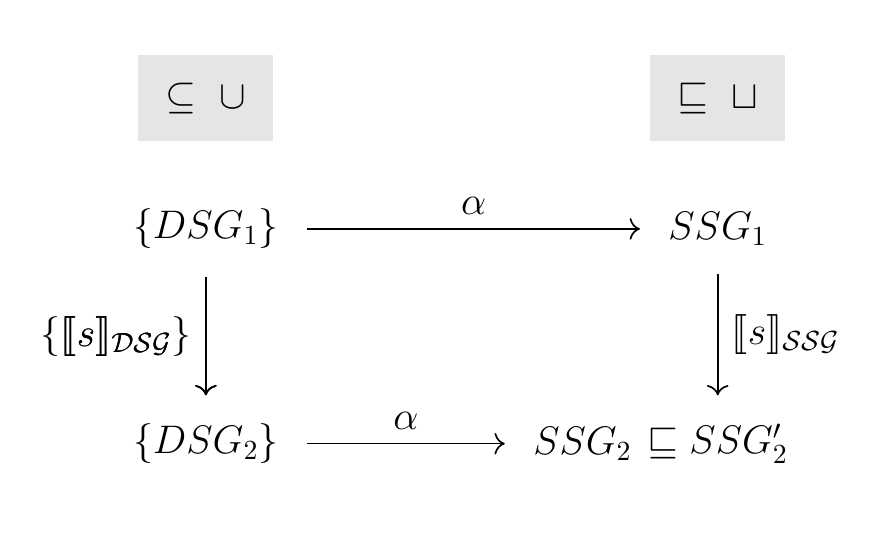
\begin{tikzpicture}[semithick,ampersand replacement=\&, >=cm to]
      \Large

      % Shape graphs
      \matrix[matrix, row sep=3em, inner sep=10pt] {
        \uncover<3->{\node[fill=gray!20!white] {$\subseteq \; \cup$};}
        \&[5em] \&[-1em]
        \uncover<4->{\node[fill=gray!20!white]
          {$\sqsubseteq \; \sqcup$};} \\[-2em]
        \node (D1) {$\phantom{\{} DSG_1 \phantom{\}}$}; \& \&
        \uncover<4->{\node (S1) {$SSG_1$};} \\
        \uncover<2->{\node (D2) {$\phantom{\{} DSG_2 \phantom{\}}$};} \&
        \uncover<5->{\node (S2) {$SSG_2$};} \&
        \uncover<6->{\node (S2bis) {$\sqsubseteq SSG'_2$};} \\
      };

      % Extra "set braces"
      \uncover<3->{
        \node at (D1) {$\{ \phantom{DSG_1} \}$};
        \node at (D2) {$\{ \phantom{DSG_2} \}$};}

      % Arrows.
      \uncover<2>{\draw[->] (D1) --
        node[left]{$\phantom{\{} \mtransformerDSG{s} \phantom{\}}$} (D2);}
      \uncover<3->{\draw[->] (D1) --
        node[left]{$\{ \mtransformerDSG{s} \}$} (D2);}
      \uncover<4->{\draw[->] (D1) -- node[above]{$\alpha$} (S1);}
      \uncover<6->{\draw[->] (S1) --
        node[right]{$\mtransformerSSG{s}$} (S2bis);}
      \uncover<5->{\draw[->] (D2) -- node[above]{$\alpha$} (S2);}
    \end{tikzpicture}
  \end{center}
\end{frame}

% 8. some examples for "abstract transformation rules" [st]SSG
%   - an easy one - new
\begin{frame}{Abstract Interpretation -- Examples}
  Allocating a new node.

  \vspace{1em}

  \begin{center}
    \begin{tikzpicture}[semithick, ampersand replacement=\&,%
      every edge/.append style={->}, >=latex]
      \Large

      %%% DSG 1 (top left) %%%
      \matrix[graph] (d1) at (-5em, 3em)
      {
        \ccons[minimum width=1em]{l1}{l_1} \&
        \ccons[minimum width=1em]{l2}{l_2} \&
        \ccons[minimum width=1em]{l3}{l_3} \\
      };

      % Selector edges.
      \path[->]
      (l1-cdr) edge (l2)
      (l2-cdr) edge (l3);

      % Variable egdes.
      \vlabel{left}{l1}{x}

      %%% SSG 1 (top right) %%%
      \matrix[graph] (s1) at (6em, 3em)
      {
        \acons{x}{\{x\}} \& \acons{e}{\emptyset} \\
      };

      % Selector edges.
      \path[->] (x-cdr) edge (e);
      \draw[->] (e-cdr) -| ++(1em, 1em) -| (e.north);

      % Variable egdes.
      \vlabel{left}{x}{x}

      %%% DSG 2 (bottom left) %%%
      \matrix[graph] (d2) at (-5em, -3em)
      {
        \ccons[minimum width=1em]{l1}{l_1} \&
        \ccons[minimum width=1em]{l2}{l_2} \&
        \ccons[minimum width=1em]{l3}{l_3} \\
        \ccons[minimum width=1em]{l4}{l_4} \\
      };

      % Selector edges.
      \path[->]
      (l1-cdr) edge (l2)
      (l2-cdr) edge (l3);

      % Variable egdes.
      \vlabel{left}{l1}{x}
      \vlabel{left}{l4}{y}

      %%% SSG 2 (bottom right) %%%
      \matrix[graph] (s2) at (6em, -3em)
      {
        \acons{x}{\{x\}} \& \acons{e}{\emptyset} \\
        \acons{y}{\{y\}} \\
      };

      % Selector edges.
      \path[->] (x-cdr) edge (e);
      \draw[->] (e-cdr) -| ++(1em, 1em) -| (e.north);

      % Variable egdes.
      \vlabel{left}{x}{x}
      \vlabel{left}{y}{y}

      %%% Transformer arrows %%%
      \vtransarrow{d1}{\transformerDSG{y := new}}{d2}
      \transarrow{d1}{$\hat{\alpha}$}{s1}
      \transarrow{d2}{$\hat{\alpha}$}{s2}
      \vtransarrow[right]{s1}{\transformerSSG{y := new}}{s2}
    \end{tikzpicture}
  \end{center}
\end{frame}

% 8. some examples for "abstract transformation rules" [st]SSG
%   - an easy one - assigning nil to fields
\begin{frame}[fragile]{Abstract Interpretation -- Examples (cont.)}
  Assigning @nil@ to a field.

  \vspace{1em}

  \begin{center}
    \begin{tikzpicture}[semithick, ampersand replacement=\&,%
      every edge/.append style={->}, >=latex]
      \Large

      %%% DSG 1 (top left) %%%
      \matrix[graph] (d1) at (-5em, 3em)
      {
        \ccons[minimum width=1em]{l1}{l_1} \&
        \ccons[minimum width=1em]{l2}{l_2} \&
        \ccons[minimum width=1em]{l3}{l_3} \&
        \ccons[minimum width=1em]{l4}{l_4} \\
      };

      % Selector edges.
      \path[->]
      (l1-cdr) edge (l2)
      (l2-cdr) edge (l3)
      (l3-cdr) edge (l4);

      % Variable egdes.
      \vlabel{left}{l1}{x}
      \vlabel{above}{l2}{y}

      %%% SSG 1 (top right) %%%
      \matrix[graph] (s1) at (6em, 3em)
      {
        \acons[minimum width=1.5em]{x}{\{x\}} \&
        \acons[minimum width=1.5em]{y}{\{y\}} \&
        \acons[minimum width=1.5em]{e}{\emptyset} \\
      };

      % Selector edges.
      \path[->]
      (x-cdr) edge (y)
      (y-cdr) edge (e);
      \draw[->] (e-cdr) -| ++(1em, 1em) -| (e.north);

      % Variable egdes.
      \vlabel{left}{x}{x}
      \vlabel{above}{y}{y}

      %%% DSG 2 (bottom left) %%%
      \matrix[graph] (d2) at (-5em, -3em)
      {
        \tcell[minimum width=1em] \\
        \ccons[minimum width=1em]{l1}{l_1} \&
        \ccons[minimum width=1em]{l2}{l_2} \&
        \ccons[minimum width=1em]{l3}{l_3} \&
        \ccons[minimum width=1em]{l4}{l_4} \\
      };

      % Selector edges.
      \path[->]
      (l2-cdr) edge (l3)
      (l3-cdr) edge (l4);

      % Variable egdes.
      \vlabel{left}{l1}{x}
      \vlabel{above}{l2}{y}

      %%% SSG 2 (bottom right) %%%
      \matrix[graph] (s2) at (6em, -3em)
      {
        \tcell[minimum width=1.5em] \\
        \acons[minimum width=1.5em]{x}{\{x\}} \&
        \acons[minimum width=1.5em]{y}{\{y\}} \&
        \acons[minimum width=1.5em]{e}{\emptyset} \\
      };

      % Selector edges.
      \path[->]
      (y-cdr) edge (e);
      \draw[->] (e-cdr) -| ++(1em, 1em) -| (e.north);

      % Variable egdes.
      \vlabel{left}{x}{x}
      \vlabel{above}{y}{y}

      %%% Transformer arrows %%%
      \vtransarrow{d1}{\transformerDSG{x.cdr := nil}}{d2}
      \transarrow{d1}{$\hat{\alpha}$}{s1}
      \transarrow{d2}{$\hat{\alpha}$}{s2}
      \vtransarrow{s1}{\transformerSSG{x.cdr := nil}}{s2}
    \end{tikzpicture}
  \end{center}
\end{frame}

% 8. some examples for "abstract transformation rules" [st]SSG
%   - assigning nil to a variable (merges nodes)
\begin{frame}[fragile]{Abstract Interpretation -- Examples (cont.)}
  Assigning @nil@ to a variable.

  \vspace{1em}

  \begin{center}
    \begin{tikzpicture}[semithick, ampersand replacement=\&,%
      every edge/.append style={->}, >=latex]
      \Large

      %%% DSG 1 (top left) %%%
      \matrix[graph] (d1) at (-5em, 3em)
      {
        \ccons[minimum width=1em]{l1}{l_1} \&
        \ccons[minimum width=1em]{l2}{l_2} \&
        \ccons[minimum width=1em]{l3}{l_3} \&
        \ccons[minimum width=1em]{l4}{l_4} \\
      };

      % Selector edges.
      \path[->]
      (l1-cdr) edge (l2)
      (l2-cdr) edge (l3)
      (l3-cdr) edge (l4);

      % Variable egdes.
      \vlabel{left}{l1}{x}
      \vlabel{above}{l2}{y}

      %%% SSG 1 (top right) %%%
      \matrix[graph] (s1) at (6em, 3em)
      {
        \acons[minimum width=1.5em]{x}{\{x\}} \&
        \acons[minimum width=1.5em]{y}{\{y\}} \&
        \acons[minimum width=1.5em]{e}{\emptyset} \\
      };

      % Selector edges.
      \path[->]
      (x-cdr) edge (y)
      (y-cdr) edge (e);
      \draw[->] (e-cdr) -| ++(1em, 1em) -| (e.north);

      % Variable egdes.
      \vlabel{left}{x}{x}
      \vlabel{above}{y}{y}

      %%% DSG 2 (bottom left) %%%
      \matrix[graph] (d2) at (-5em, -3em)
      {
        \ccons[minimum width=1em]{l1}{l_1} \&
        \ccons[minimum width=1em]{l2}{l_2} \&
        \ccons[minimum width=1em]{l3}{l_3} \&
        \ccons[minimum width=1em]{l4}{l_4} \\
      };

      % Selector edges.
      \path[->]
      (l1-cdr) edge (l2)
      (l2-cdr) edge (l3)
      (l3-cdr) edge (l4);

      % Variable egdes.
      \vlabel{left}{l1}{x}

      %%% SSG 2 (bottom right) %%%
      \matrix[graph] (s2) at (6em, -3em)
      {
        \acons[minimum width=1.5em]{x}{\{x\}} \&
        \tcell[minimum width=1.5em] \&
        \acons[minimum width=1.5em]{e}{\emptyset} \\
      };

      % Selector edges.
      \path[->] (x-cdr) edge (e);
      \draw[->] (e-cdr) -| ++(1em, 1em) -| (e.north);

      % Variable egdes.
      \vlabel{left}{x}{x}

      %%% Transformer arrows %%%
      \vtransarrow{d1}{\transformerDSG{y := nil}}{d2}
      \transarrow{d1}{$\hat{\alpha}$}{s1}
      \transarrow{d2}{$\hat{\alpha}$}{s2}
      \vtransarrow[right]{s1}{\transformerSSG{y := nil}}{s2}
    \end{tikzpicture}
  \end{center}
\end{frame}


% 8. some examples for "abstract transformation rules" [st]SSG
%   - materialisation
\begin{frame}{Abstract Interpretation -- Examples (cont.)}
  Materialising a node $n_y$ from the summary node $n_\emptyset$.

  \vspace{1em}

  \begin{center}
    \begin{tikzpicture}[semithick, ampersand replacement=\&,%
      every edge/.append style={->}, >=latex]
      \Large

      %%% DSG 1 (top left) %%%
      \matrix[graph] (d1) at (-5em, 3em)
      {
        \ccons[minimum width=1em]{l1}{l_1} \&
        \ccons[minimum width=1em]{l2}{l_2} \&
        \ccons[minimum width=1em]{l3}{l_3} \&
        \ccons[minimum width=1em]{l4}{l_4} \\
      };

      % Selector edges.
      \path[->]
      (l1-cdr) edge (l2)
      (l2-cdr) edge (l3)
      (l3-cdr) edge (l4);

      % Variable egdes.
      \vlabel{left}{l1}{x}

      %%% SSG 1 (top right) %%%
      \matrix[graph] (s1) at (6em, 3em)
      {
        \acons[minimum width=1.5em]{x}{\{x\}} \&
        \tcell[minimum width=1.5em] \&
        \acons[minimum width=1.5em]{e}{\emptyset} \\
      };

      % Selector edges.
      \path[->] (x-cdr) edge (e);
      \draw[->] (e-cdr) -| ++(1em, 1em) -| (e.north);

      % Variable egdes.
      \vlabel{left}{x}{x}

      %%% DSG 2 (bottom left) %%%
      \matrix[graph] (d2) at (-5em, -3em)
      {
        \tcell[minimum width=1em] \\
        \ccons[minimum width=1em]{l1}{l_1} \&
        \ccons[minimum width=1em]{l2}{l_2} \&
        \ccons[minimum width=1em]{l3}{l_3} \&
        \ccons[minimum width=1em]{l4}{l_4} \\
      };

      % Selector edges.
      \path[->]
      (l1-cdr) edge (l2)
      (l2-cdr) edge (l3)
      (l3-cdr) edge (l4);

      % Variable egdes.
      \vlabel{left}{l1}{x}
      \vlabel{above}{l2}{y}

      %%% SSG 2 (bottom right) %%%
      \matrix[graph] (s2) at (6em, -3em)
      {
        \tcell[minimum width=1em] \\
        \acons[minimum width=1.5em]{x}{\{x\}} \&
        \acons[minimum width=1.5em]{y}{\{y\}} \&
        \acons[minimum width=1.5em]{e}{\emptyset} \\
      };

      % Selector edges.
      \path[->]
      (x-cdr) edge (y)
      (y-cdr) edge (e);
      \draw[->] (e-cdr) -| ++(1em, 1em) -| (e.north);

      % Variable egdes.
      \vlabel{left}{x}{x}
      \vlabel{above}{y}{y}

      %%% Transformer arrows %%%
      \vtransarrow{d1}{\transformerDSG{y := x.cdr}}{d2}
      \transarrow{d1}{$\hat{\alpha}$}{s1}
      \transarrow{d2}{$\hat{\alpha}$}{s2}
      \vtransarrow{s1}{\transformerSSG{y := x.cdr}}{s2}
    \end{tikzpicture}
  \end{center}
\end{frame}

% 8. some examples for "abstract transformation rules" [st]SSG
%   - variable assignment
\begin{frame}{Abstract Interpretation -- Examples (cont.)}

  \vspace{.5em}
  Variable assignment.
  \vspace{.5em}

  \begin{center}
    \begin{tikzpicture}[semithick, ampersand replacement=\&,%
      every edge/.append style={->}, >=latex]
      \Large

      %%% DSG 1 (top left) %%%
      \matrix[graph, row sep=1ex, left delimiter=\{,
      right delimiter=\}] (d1) at (-6em, 4em)
      {
        \tcell[minimum width=.25em, minimum height=.25em] \\
        \&
        \ccons[minimum width=1em]{l1-1}{l_1} \&
        \ccons[minimum width=1em]{l2-1}{l_2} \&
        \ccons[minimum width=1em]{l3-1}{l_3} \&
        \ccons[minimum width=1em]{l4-1}{l_4} \\
        \&
        \ccons[minimum width=1em]{l1-2}{l_1} \&
        \ccons[minimum width=1em]{l2-2}{l_2} \&
        \ccons[minimum width=1em]{l3-2}{l_3} \&
        \ccons[minimum width=1em]{l4-2}{l_4} \\
      };

      % Selector edges.
      \path[->]
      (l1-1-cdr) edge (l2-1)
      (l2-1-cdr) edge (l3-1)
      (l3-1-cdr) edge (l4-1)
      (l1-2-cdr) edge (l2-2)
      (l2-2-cdr) edge (l3-2)
      (l3-2-cdr) edge (l4-2);

      % Variable egdes.
      \vlabel{left}{l1-1}{x}
      \vlabel{above}{l2-1}{y}
      \vlabelwy{l1-2}{x}{.5ex}
      \vlabelwy{l1-2}{y}{-.5ex}

      %%% SSG 1 (top right) %%%
      \matrix[graph] (s1) at (6em, 4em)
      {
        \acons[minimum width=1.5em]{x}{\{x\}} \\
        \acons[minimum width=1.5em]{xy}{\{x,y\}} \&
        \acons[minimum width=1.5em]{y}{\{y\}} \&
        \acons[minimum width=1.5em]{e}{\emptyset} \\
      };

      % Selector edges.
      \path[->]
      (x-cdr) edge (y)
      (xy-cdr) edge (y)
      (y-cdr) edge (e);
      \draw[->] (e-cdr) -| ++(1em, 1em) -| (e.north);

      % Variable egdes.
      \vlabel{left}{x}{x}
      \vlabel{above}{y}{y}
      \vlabelwy{xy}{x}{.5ex}
      \vlabelwy{xy}{y}{-.5ex}

      %%% DSG 2 (bottom left) %%%
      \matrix[graph, row sep=1ex, left delimiter=\{,
      right delimiter=\}] (d2) at (-6em, -4em)
      {
        \tcell[minimum width=.25em, minimum height=.25em] \\
        \&
        \ccons[minimum width=1em]{l1-1}{l_1} \&
        \ccons[minimum width=1em]{l2-1}{l_2} \&
        \ccons[minimum width=1em]{l3-1}{l_3} \&
        \ccons[minimum width=1em]{l4-1}{l_4} \\
        \&
        \ccons[minimum width=1em]{l1-2}{l_1} \&
        \ccons[minimum width=1em]{l2-2}{l_2} \&
        \ccons[minimum width=1em]{l3-2}{l_3} \&
        \ccons[minimum width=1em]{l4-2}{l_4} \\
      };

      % Selector edges.
      \path[->]
      (l1-1-cdr) edge (l2-1)
      (l2-1-cdr) edge (l3-1)
      (l3-1-cdr) edge (l4-1)
      (l1-2-cdr) edge (l2-2)
      (l2-2-cdr) edge (l3-2)
      (l3-2-cdr) edge (l4-2);

      % Variable egdes.
      \vlabel{left}{l1-1}{x}
      \vlabelnx{l2-1}{y}{-.5ex}
      \vlabelnx{l2-1}{z}{.5ex}
      \vlabelwy{l1-2}{x}{.75ex}
      \vlabel{left}{l1-2}{y}
      \vlabelwy{l1-2}{z}{-.75ex}

      %%% SSG 2 (bottom right) %%%
      \matrix[graph] (s2) at (6em, -4em)
      {
        \tcell[minimum width=1.5em, minimum height=0.25em] \\
        \acons[minimum width=1.5em]{x}{\{x\}} \\
        \acons[minimum width=1.5em]{xyz}{\{x,y,z\}} \&
        \acons[minimum width=1.5em]{yz}{\{y,z\}} \&
        \acons[minimum width=1.5em]{e}{\emptyset} \\
      };

      % Selector edges.
      \path[->]
      (x-cdr) edge (yz)
      (xyz-cdr) edge (yz)
      (yz-cdr) edge (e);
      \draw[->] (e-cdr) -| ++(1em, 1em) -| (e.north);

      % Variable egdes.
      \vlabel{left}{x}{x}
      \vlabelnx{yz}{y}{-.5ex}
      \vlabelnx{yz}{z}{.5ex}
      \vlabelwy{xyz}{x}{.75ex}
      \vlabel{left}{xyz}{y}
      \vlabelwy{xyz}{z}{-.75ex}

      %%% Transformer arrows %%%
      \vtransarrow{d1}{\transformerDSG{z := y}}{d2}
      \transarrow{d1}{$\alpha$}{s1}
      \transarrow{d2}{$\alpha$}{s2}
      \vtransarrow[right]{s1}{\transformerSSG{z := y}}{s2}
    \end{tikzpicture}
  \end{center}
\end{frame}

% 8. some examples for "abstract transformation rules" [st]SSG
%   - strong nullification
\begin{frame}{Abstract Interpretation -- Examples (cont.)}

  \vspace{.5em}
  Strong nullification.
  \vspace{.5em}

  \begin{center}
    \begin{tikzpicture}[semithick, ampersand replacement=\&,%
      every edge/.append style={->}, >=latex]
      \Large

      %%% DSG 1 (top left) %%%
      \matrix[graph, row sep=1ex, left delimiter=\{,
      right delimiter=\}] (d1) at (-6em, 4em)
      {
        \tcell[minimum width=.25em, minimum height=.25em] \\
        \&
        \ccons[minimum width=1em]{l1-1}{l_1} \&
        \ccons[minimum width=1em]{l2-1}{l_2} \&
        \ccons[minimum width=1em]{l3-1}{l_3} \&
        \ccons[minimum width=1em]{l4-1}{l_4} \\
        \&
        \ccons[minimum width=1em]{l1-2}{l_1} \&
        \ccons[minimum width=1em]{l2-2}{l_2} \&
        \ccons[minimum width=1em]{l3-2}{l_3} \&
        \ccons[minimum width=1em]{l4-2}{l_4} \\
      };

      % Selector edges.
      \path[->]
      (l1-1-cdr) edge (l2-1)
      (l2-1-cdr) edge (l3-1)
      (l3-1-cdr) edge (l4-1)
      (l1-2-cdr) edge (l2-2)
      (l2-2-cdr) edge (l3-2)
      (l3-2-cdr) edge (l4-2);

      % Variable egdes.
      \vlabel{left}{l1-1}{x}
      \vlabel{above}{l2-1}{y}
      \vlabelwy{l1-2}{x}{.5ex}
      \vlabelwy{l1-2}{y}{-.5ex}

      %%% SSG 1 (top right) %%%
      \matrix[graph] (s1) at (6em, 4em)
      {
        \acons[minimum width=1.5em]{x}{\{x\}} \\
        \acons[minimum width=1.5em]{xy}{\{x,y\}} \&
        \acons[minimum width=1.5em]{y}{\{y\}} \&
        \acons[minimum width=1.5em]{e}{\emptyset} \\
      };

      % Selector edges.
      \path[->]
      (x-cdr) edge (y)
      (xy-cdr) edge (y)
      (y-cdr) edge (e);
      \draw[->] (e-cdr) -| ++(1em, 1em) -| (e.north);

      % Variable egdes.
      \vlabel{left}{x}{x}
      \vlabel{above}{y}{y}
      \vlabelwy{xy}{x}{.5ex}
      \vlabelwy{xy}{y}{-.5ex}

      %%% DSG 2 (bottom left) %%%
      \matrix[graph, row sep=1ex, left delimiter=\{,
      right delimiter=\}] (d2) at (-6em, -4em)
      {
        \tcell[minimum width=.25em, minimum height=.25em] \\
        \&
        \ccons[minimum width=1em]{l1-1}{l_1} \&
        \ccons[minimum width=1em]{l2-1}{l_2} \&
        \ccons[minimum width=1em]{l3-1}{l_3} \&
        \ccons[minimum width=1em]{l4-1}{l_4} \\
        \&
        \ccons[minimum width=1em]{l1-2}{l_1} \&
        \ccons[minimum width=1em]{l2-2}{l_2} \&
        \ccons[minimum width=1em]{l3-2}{l_3} \&
        \ccons[minimum width=1em]{l4-2}{l_4} \\
      };

      % Selector edges.
      \path[->]
      (l2-1-cdr) edge (l3-1)
      (l3-1-cdr) edge (l4-1)
      (l2-2-cdr) edge (l3-2)
      (l3-2-cdr) edge (l4-2);

      % Variable egdes.
      \vlabel{left}{l1-1}{x}
      \vlabel{above}{l2-1}{y}
      \vlabelwy{l1-2}{x}{.5ex}
      \vlabelwy{l1-2}{y}{-.5ex}

      %%% SSG 2 (bottom right) %%%
      \matrix[graph] (s2) at (6em, -4em)
      {
        \tcell[minimum width=1.5em, minimum height=0.25em] \\
        \acons[minimum width=1.5em]{x}{\{x\}} \\
        \acons[minimum width=1.5em]{xy}{\{x,y\}} \&
        \acons[minimum width=1.5em]{y}{\{y\}} \&
        \acons[minimum width=1.5em]{e}{\emptyset} \\
      };

      % Selector edges.
      \path[->] (y-cdr) edge (e);
      \draw[->] (e-cdr) -| ++(1em, 1em) -| (e.north);

      % Variable egdes.
      \vlabel{left}{x}{x}
      \vlabel{above}{y}{y}
      \vlabelwy{xy}{x}{.5ex}
      \vlabelwy{xy}{y}{-.5ex}

      %%% Transformer arrows %%%
      \vtransarrow{[xshift=1em]d1}{\transformerDSG{x.cdr := nil}}{%
        [xshift=1em]d2}
      \transarrow{d1}{$\alpha$}{s1}
      \transarrow{d2}{$\alpha$}{s2}
      \vtransarrow{s1}{\transformerSSG{x.cdr := nil}}{s2}
    \end{tikzpicture}
  \end{center}
\end{frame}


\begin{frame}[fragile]{List Insertion -- Normalisation}
  \begin{columns}[T]
	  \column{.5\textwidth}
	  \begin{onlyenv}<1>
	  \begin{lstlisting}[mathescape]
	  // x points to an unshared list
	  
	  y := x
	  while y.cdr $ \neq $ nil $ \wedge \ldots $ do

	    z := y.cdr

	    y := z
	  od

	  t := y.cdr

	  e.cdr := t

	  y.cdr := e
	  t := nil
	  z := nil
	  e := nil
	  y := nil
	  \end{lstlisting}
	  \end{onlyenv}
	  \begin{onlyenv}<2->
	  \begin{lstlisting}[mathescape]
	  // x points to an unshared list
	  @y := nil@
	  y := x
	  while y.cdr $ \neq $ nil $ \wedge \ldots $ do
	    @z := nil@
	    z := y.cdr
	    @y := nil@
	    y := z
	  od
	  @t := nil@
	  t := y.cdr
	  @e.cdr := nil@
	  e.cdr := t
	  @y.cdr := nil@
	  y.cdr := e
	  t := nil
	  z := nil
	  e := nil
	  y := nil
	  \end{lstlisting}
    \end{onlyenv}
        \column{.5\textwidth}
        \pause\pause
        \begin{tikzpicture}[ampersand replacement=\&, >=latex,
          level 2/.style={onslide=<-3>{transparent}}]
        
          \tiny
          \matrix[row sep=.75em] {
            \stmt{1}{y := nil} \\
            \stmt{2}{y := x} \\
            \stmt{3}{} \\
            \stmt{4}{z := nil} \\
            \stmt{5}{z := y.cdr} \\
            \stmt{6}{y := nil} \\
            \stmt{7}{y := z} \\
            \stmt{8}{t := nil} \\
            \stmt{9}{t := y.cdr} \\
            \stmt{10}{e.cdr := nil} \\
            \stmt{11}{e.cdr := t} \\
            \stmt{12}{y.cdr := nil} \\
            \stmt{13}{y.cdr := e} \\
            \stmt{14-18}{...} \\
          };
          \path[->]
          (v1.north) +(0,+1em) edge (v1)
          (v1) edge (v2)
          (v2) edge (v3)
          (v3) edge (v4)
          (v4) edge (v5)
          (v5) edge (v6)
          (v6) edge (v7)
          (v8) edge (v9)
          (v9) edge (v10)
          (v10) edge (v11)
          (v11) edge (v12)
          (v12) edge (v13)
          (v13) edge (v14-18);
          \draw[->] ([yshift=.5ex]v3.east) -- +(2em, 0) |- (v8);
          \draw[->] (v7.east) -- +(1em, 0) |- ([yshift=-.5ex]v3);

          \begin{scope}[level 2]
	          \stmtgroup{v1}{v2}{init}
	          %\stmtgroup{v3}{v3}{branch}
	          \stmtgroup{v4}{v7}{loop}
	          \stmtgroup{v8}{v14-18}{rest}
	        \end{scope}
        \end{tikzpicture}
        \pause
  \end{columns}
\end{frame}

\begin{frame}[fragile]{Sharing}
  \only<1>{

  From $v_1$ to $v_{11}$ \textit{without entering} the loop. \\
  Executing \transformer{e.cdr := nil}{} -- $n_{\{t\}}$ is \textbf{not} shared.
  %\vspace{1.5em} % TODO need better alignment (vertical & horizontal)

  \begin{center}
    \begin{tikzpicture}[semithick,
%      level 1/.style={onslide=<-0>{transparent}},
%      level 2/.style={onslide=<-1>{transparent}},
%      level 3/.style={onslide=<-2>{transparent}},
      ampersand replacement=\&, every edge/.append style={->}, >=latex]
      \Large

      % Fig. 8/9, at vertex v11 (before) when loop not executed:
%      \begin{scope}[level 1]
	      \matrix[graph, column sep=1em] (g1)
	      {
	         \ntcell{x}      \& \ntcell{yz}          \& \acons{t}{\{t\}} \& \acons{phi}{\emptyset} \\
	                         \& \acons{xy}{\{x, y\}} \& \acons{e}{\{e\}} \&                        \\
	      };

	      % Selector edges.
	      \path[->]
	      (t-cdr) edge (phi)
	      (xy-cdr) edge (t.south west);
	      % loop for phi
	      \draw[->] (phi-cdr) -| ++(1em, 1em) -| (phi.north);
	      % invisible loops
	      \draw[->, transparent] (x-cdr) -| ++(0, 2em) -| ([xshift=-1ex]phi.north);

	      % Variable egdes.
	      \vlabelwy{xy}{x}{1.5mm}
	      \vlabelwy{xy}{y}{-1.5mm}
	      \vlabelwy{t}{t}{1.5mm}
	      \vlabelwy{e}{e}{0mm}
              % Invisible variable edge.
              \node[labelnode, left=of x] {$\phantom{x}$};
%      \end{scope}
    \end{tikzpicture}
  \end{center}
  \begin{tikzpicture}[ampersand replacement=\&, >=latex]
      \tiny
      \matrix[row sep=1.5em] {
        \stmtmini{init} \\
        \stmtmini{loop} \\
        \stmtmini{rest} \\
      };
      
      \path[ImportantPath, ->, thick] (init.north) +(0,+2em) edge (init);
      \draw[ImportantPath, ->, thick] (init.east) -- +(2em, 0) |- (rest);
  \end{tikzpicture}
  }

  \only<2>{

  From $v_1$ to $v_{11}$ \textit{through} the loop. \\
  Executing \transformer{e.cdr := nil}{} -- $n_{\{t\}}$ is \textbf{not} shared.

  \begin{center}
    \begin{tikzpicture}[semithick,
%      level 1/.style={onslide=<-0>{transparent}},
%      level 2/.style={onslide=<-1>{transparent}},
%      level 3/.style={onslide=<-2>{transparent}},
      ampersand replacement=\&, every edge/.append style={->}, >=latex]
      \Large

      % Fig. 8/9, at vertex v11 (before) when loop is executed:
%      \begin{scope}[level 1]
	      \matrix[graph, column sep=1em] (g1)
	      {
	        \acons{x}{\{x\}} \& \acons{yz}{\{y, z\}} \& \acons{t}{\{t\}} \& \acons{phi}{\emptyset} \\
	                         \&                      \& \acons{e}{\{e\}} \&                        \\
	      };


	      % Selector edges.
	      \path[->]
	      (t-cdr) edge (phi)
	      (x-cdr) edge (yz)
	      (yz-cdr) edge (t);
	      % loops
	      \draw[->] (x-cdr) -| ++(0, 2em) -| ([xshift=-1ex]phi.north);
	      \draw[->] (phi-cdr) -| ++(1em, 1em) -| (phi.north);
	      \draw[->] (phi-cdr) -| ++(0, 1.5em) -| (yz.north);
	      \draw[->] (t-cdr) -| ++(0, 1em) -| ([xshift=1ex]yz.north);

	      % Variable egdes.
	      \vlabelwy{x}{x}{0mm}
	      \vlabelwy{yz}{y}{1.5mm}
	      \vlabelwy{yz}{z}{-1.5mm}
	      \vlabelwy{t}{t}{1.5mm}
	      \vlabelwy{e}{e}{0mm}
%      \end{scope}
    \end{tikzpicture}
  \end{center}
  \begin{tikzpicture}[ampersand replacement=\&, >=latex]
      \tiny
      \matrix[row sep=1.5em] {
          \stmtmini{init} \\
          \stmtmini{loop} \\
          \stmtmini{rest} \\
        };
        
        \path[ImportantPath, ->, thick] 
            (init.north) +(0,+2em) edge (init)
            (init) edge (loop)
            (loop) edge (rest);
        \draw[ImportantPath, ->, thick] (loop.east) -| ++(1em, 2em) -| ([xshift=1em]loop.north);
    \end{tikzpicture}
  }

  \only<3>{

  From $v_1$ to $v_{11}$ by all possible paths. \\
  Executing \transformer{e.cdr := nil}{} -- $n_{\{t\}}$ is still \textbf{not} shared.

  \begin{center}
    \begin{tikzpicture}[semithick,
%      level 1/.style={onslide=<-0>{transparent}},
%      level 2/.style={onslide=<-1>{transparent}},
%      level 3/.style={onslide=<-2>{transparent}},
      ampersand replacement=\&, every edge/.append style={->}, >=latex]
      \Large

      % Fig. 8/9, at vertex v11 (before) for all paths:
%      \begin{scope}[level 1]
	      \matrix[graph, column sep=1em] (g1)
	      {
	        \acons{x}{\{x\}} \& \acons{yz}{\{y, z\}} \& \acons{t}{\{t\}} \& \acons{phi}{\emptyset} \\
	                         \& \acons{xy}{\{x, y\}} \& \acons{e}{\{e\}} \&                        \\
	      };


	      % Selector edges.
	      \path[->]
	      (t-cdr) edge (phi)
	      (x-cdr) edge (yz)
	      (xy-cdr) edge (t.south west)
	      (yz-cdr) edge (t);
	      % loops
	      \draw[->] (x-cdr) -| ++(0, 2em) -| ([xshift=-1ex]phi.north);
	      \draw[->] (phi-cdr) -| ++(1em, 1em) -| (phi.north);
	      \draw[->] (phi-cdr) -| ++(0, 1.5em) -| (yz.north);
	      \draw[->] (t-cdr) -| ++(0, 1em) -| ([xshift=1ex]yz.north);

	      % Variable egdes.
	      \vlabelwy{x}{x}{0mm}
	      \vlabelwy{xy}{x}{1.5mm}
	      \vlabelwy{xy}{y}{-1.5mm}
	      \vlabelwy{yz}{y}{1.5mm}
	      \vlabelwy{yz}{z}{-1.5mm}
	      \vlabelwy{t}{t}{1.5mm}
	      \vlabelwy{e}{e}{0mm}
%      \end{scope}
    \end{tikzpicture}
  \end{center}
  \begin{tikzpicture}[ampersand replacement=\&, >=latex]
      \tiny
      \matrix[row sep=1.5em] {
          \stmtmini{init} \\
          \stmtmini{loop} \\
          \stmtmini{rest} \\
        };
        
      \path[ImportantPath, ->, thick] 
          (init.north) +(0,+2em) edge (init)
          (init) edge (loop)
          (loop) edge (rest);

      \draw[ImportantPath, ->, thick] (init.east) -- +(2em, 0) |- (rest);
      \draw[ImportantPath, ->, thick] (loop.east) -| ++(1em, 2em) -| ([xshift=1em]loop.north);
    \end{tikzpicture}
  }

  \only<4>{

  From $v_1$ to $v_{12}$ by all possible paths. \\
  Executing \transformer{e.cdr := t}{} -- $n_{\{t\}}$ \textbf{is} shared.

  \begin{center}
    \begin{tikzpicture}[semithick,
%      level 1/.style={onslide=<-0>{transparent}},
%      level 2/.style={onslide=<-1>{transparent}},
%      level 3/.style={onslide=<-2>{transparent}},
      ampersand replacement=\&, every edge/.append style={->}, >=latex]
      \Large

      % Fig. 8/9, at vertex v12 (before) for all paths:
%      \begin{scope}[level 1]
	      \matrix[graph, column sep=1em] (g1)
	      {
	        \acons{x}{\{x\}} \& \acons{yz}{\{y, z\}} \& \scons{t}{\{t\}} \& \acons{phi}{\emptyset} \\
	                         \& \acons{xy}{\{x, y\}} \& \acons{e}{\{e\}} \&                        \\
	      };


	      % Selector edges.
	      \path[->]
	      (t-cdr) edge (phi)
	      (x-cdr) edge (yz)
	      (xy-cdr) edge (t.south west)
	      (yz-cdr) edge (t)
	      (e-cdr) edge[RubineRed] ([xshift=1ex]t.south);
	      % loops
	      \draw[->] (x-cdr) -| ++(0, 2em) -| ([xshift=-1ex]phi.north);
	      \draw[->] (phi-cdr) -| ++(1em, 1em) -| (phi.north);
	      \draw[->] (phi-cdr) -| ++(0, 1.5em) -| (yz.north);
	      \draw[->] (t-cdr) -| ++(0, 1em) -| ([xshift=1ex]yz.north);

	      % Variable egdes.
	      \vlabelwy{x}{x}{0mm}
	      \vlabelwy{xy}{x}{1.5mm}
	      \vlabelwy{xy}{y}{-1.5mm}
	      \vlabelwy{yz}{y}{1.5mm}
	      \vlabelwy{yz}{z}{-1.5mm}
	      \vlabelwy{t}{t}{1.5mm}
	      \vlabelwy{e}{e}{0mm}
%      \end{scope}
    \end{tikzpicture}
  \end{center}

  \begin{tikzpicture}[ampersand replacement=\&, >=latex]
    \tiny
    \matrix[row sep=1.5em] {
        \stmtmini{init} \\
        \stmtmini{loop} \\
        \stmtmini{rest} \\
      };
      
    \path[ImportantPath, ->, thick] 
        (init.north) +(0,+2em) edge (init)
        (init) edge (loop)
        (loop) edge (rest);

    \draw[ImportantPath, ->, thick] (init.east) -- +(2em, 0) |- (rest);
    \draw[ImportantPath, ->, thick] (loop.east) -| ++(1em, 2em) -| ([xshift=1em]loop.north);
  \end{tikzpicture}
  }

  \only<5>{

  From $v_1$ to $v_{13}$ by all possible paths. \\
  Executing \transformer{y.cdr := nil}{} -- \textbf{strong nullification}.$\phantom{n_{\set{t}}}$

  \begin{center}
    \begin{tikzpicture}[semithick,
%      level 1/.style={onslide=<-0>{transparent}},
%      level 2/.style={onslide=<-1>{transparent}},
%      level 3/.style={onslide=<-2>{transparent}},
      ampersand replacement=\&, every edge/.append style={->}, >=latex]
      \Large

      % Fig. 8/9, at vertex v13 (before) for all paths:
%      \begin{scope}[level 1]
	      \matrix[graph, column sep=1em] (g1)
	      {
	        \acons{x}{\{x\}} \& \acons{yz}{\{y, z\}} \& \acons{t}{\{t\}} \& \acons{phi}{\emptyset} \\
	                         \& \acons{xy}{\{x, y\}} \& \acons{e}{\{e\}} \&                        \\
	      };


	      % Selector edges.
	      \path[->]
	      (t-cdr) edge (phi)
	      (x-cdr) edge (yz)
	      (xy-cdr) edge[LightGrey] (t.south west)
	      (yz-cdr) edge[LightGrey] (t)
	      (e-cdr) edge ([xshift=1ex]t.south);
	      % loops
	      \draw[->] (x-cdr) -| ++(0, 2em) -| ([xshift=-1ex]phi.north);
	      \draw[->] (phi-cdr) -| ++(1em, 1em) -| (phi.north);
	      \draw[->] (phi-cdr) -| ++(0, 1.5em) -| (yz.north);
	      \draw[->] (t-cdr) -| ++(0, 1em) -| ([xshift=1ex]yz.north);

	      % Variable egdes.
	      \vlabelwy{x}{x}{0mm}
	      \vlabelwy{xy}{x}{1.5mm}
	      \vlabelwy{xy}{y}{-1.5mm}
	      \vlabelwy{yz}{y}{1.5mm}
	      \vlabelwy{yz}{z}{-1.5mm}
	      \vlabelwy{t}{t}{1.5mm}
	      \vlabelwy{e}{e}{0mm}
%      \end{scope}
    \end{tikzpicture}
  \end{center}
  
    \begin{tikzpicture}[ampersand replacement=\&, >=latex]
      \tiny
      \matrix[row sep=1.5em] {
          \stmtmini{init} \\
          \stmtmini{loop} \\
          \stmtmini{rest} \\
        };
        
      \path[ImportantPath, ->, thick] 
          (init.north) +(0,+2em) edge (init)
          (init) edge (loop)
          (loop) edge (rest);
  
      \draw[ImportantPath, ->, thick] (init.east) -- +(2em, 0) |- (rest);
      \draw[ImportantPath, ->, thick] (loop.east) -| ++(1em, 2em) -| ([xshift=1em]loop.north);
    \end{tikzpicture}
  }
\end{frame}

\begin{frame}[fragile]{Extensions}
  \begin{description}
  \item[Merging Shape-Nodes] to avoid a huge number of nodes ($\leq 2^{|PVar|}$), a widening operator can be introduced.
  \item[Finding Aliases and Sharing] testing whether $x$ and $y$ are aliases at some point of the program can be extended to test whether two paths can alias by introducing two extra variables.
  \item[Interprocedural Analysis] \textit{shape-graph-transformations} can be introduced to accurately model procedures.
  \item[Representing Definitely Circular Structures] with extra special nodes ($n_{atom}, n_{nil}, n_{uninit}$), definitely cyclic data structures can be modelled.
  \end{description}
\end{frame}
\fi

\if0
\begin{frame}[fragile,t]{Graph example}
  \vspace{-0.5em}\uncover<2-4>{ % this diagram is visible in slides 2-4.
  \begin{center}
    \begin{tikzpicture}[semithick,
      % The "level X" styles below can be used to uncover graphs or
      % parts thereof across slides.
      level 2/.style={onslide=<-2>{transparent}},
      level 3/.style={onslide=<-3>{transparent}},
      ampersand replacement=\&, every edge/.append style={->}, >=latex]
      \Large % <-- determines scale of diagram. try \LARGE, \Huge, \small...


      % Matrix for arranging graph naodes.  You can set the overall
      % spacing through "row sep" and "column sep" or add and remove
      % horizontal or vertical space in brackets after \& and \\.
      \matrix[graph, column sep=1em] (g1) %<-- general column spacing
      {
        \ccons[minimum width=1em]{l1}{l_1} \&
        \ccons[minimum width=1em]{l2}{l_2} \&[-.5em] % <-- remove space
        \ccons[minimum width=1em]{l3}{l_3} \\
      };

      % Selector edges.
      \path[->]
      (l1-cdr) edge (l2)
      (l2-cdr) edge (l3);

      % Variable egdes.
      \vlabel{left}{l1}{x}

      % This second graph won't be shown until slide 3.
      \begin{scope}[yshift=-4em, level 2]
        \matrix[graph] (g2) %
        {
          \acons{x}{\{x\}} \& \\
          \acons{xt1}{\{x, t_1\}} \&
          \scons{e}{\emptyset}\\[.5em] % <-- extra space
          \acons{y}{\{y\}} \& \acons{t}{\{t\}}\\
        };

        % Selector edges.
        \path[->] % Normal edges.
        (x-cdr) edge (e.north west)
        (xt1-cdr) edge (e)
        (y-cdr) edge (t);
        % A loop.  Not visible until slide 4.
        \draw[->, level 3] (e-cdr) -| ++(1em, 1em) -| (e.north);

        % Variable egdes.
        \vlabel{left}{x}{x}
        \vlabel{yshift=1ex,left}{xt1}{x}
        \vlabel{yshift=-1ex,left}{xt1}{t_1}
        \vlabel{left}{y}{y}
        \vlabel{right}{t}{t}
      \end{scope}
    \end{tikzpicture}
  \end{center}}
  The diagram above won't show up until slide 2.
\end{frame}
\fi



%\begin{frame}[fragile]{Some citations and maths}
%  The \emph{Probability Monad} is a variant of the @List@
%  monad.\footnote{See e.g.\ \cite{RamseyP2002popl,Gibbons2012utp}}
%
%  \begin{lstlisting}
%  type Dist[+A] = List[(A, Double)]
%  final case class Rand[+A](dist: Dist[A]) {
%    // Monadic "bind"
%    def flatMap[B](f: A => Rand[B]): Rand[B] = Rand(
%      for ((v, p) <- dist; (w, q) <- f(v).dist)
%      yield (w, q * p))
%    ...
%  }
%  \end{lstlisting}
%  Computations are sequenced using the \emph{chain rule}:
%  \[
%  \Pr\{ f(X) = y \} = \sum_{x} \Pr\{ f(X) = y \,|\, X = x \} \Pr\{ X =
%  x \}
%  \]
%\end{frame}

\begin{frame}{Thank you!}
  \begin{center}
    \Huge Questions?
  \end{center}
\end{frame}

%%%  Backup slides  %%%

%\appendix
%\newcounter{finalframe}
%\setcounter{finalframe}{\value{framenumber}}
%
%\begin{frame}[noframenumbering]
%  \begin{center}
%    \emph{\LARGE Additional slides}
%  \end{center}
%\end{frame}
%
%\begin{frame}[fragile]{The \texttt{grassModel} in Odds}
%  \setcounter{framenumber}{\value{finalframe}}%
%  \begin{lstlisting}
%  trait CodeExample extends Stuff {
%    def grassModel: Rand[Boolean] = {
%      val rain       = flip(0.3)
%      val sprinkler  = flip(0.5)
%      val grassIsWet =
%        flip(0.9) && rain      ||
%        flip(0.8) && sprinkler ||
%        flip(0.1)
%      if (grassIsWet) rain else never
%    }
%  }
%  \end{lstlisting}
%\end{frame}
%
%\begin{frame}[noframenumbering]{Quotes and graphics}
%  The Monty Hall problem:
%  \begin{quote}
%    Suppose you're on a game show, and you're given the choice of
%    three doors: Behind one door is a car; behind the others,
%    goats. You pick a door, say No. 1, and the host, who knows what's
%    behind the doors, opens another door, say No. 3, which has a
%    goat. He then says to you, "Do you want to pick door No. 2?" Is it
%    to your advantage to switch your choice?
%
%    \hfill{\em \cite{vosSavant1990monty}}
%  \end{quote}
%  \begin{center}
%    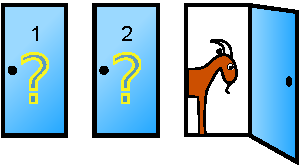
\includegraphics[height=2cm]{img/monty/Monty_open_door}
%  \end{center}
%\end{frame}


%%% Bibliography

%\bibliography{monty,biblio}
%\bibliographystyle{apalike}

\end{document}


